% ---------------------------------------------------------------------
%  CHƯƠNG 4 — THIẾT KẾ HỆ THỐNG
% ---------------------------------------------------------------------
\chapter{Thiết kế hệ thống}
\label{ch:thietke}

\begin{muctieu}
Chương này trình bày thiết kế hệ thống FoodAI, bao gồm các sơ đồ Use Case và tuần tự, kiến trúc phân tầng, mô hình cơ sở dữ liệu quan hệ và giải thuật gợi ý món ăn kết hợp AI tạo sinh với bộ lọc ngữ nghĩa.
\end{muctieu}

\section{Đặc tả Use Case và Sơ đồ tuần tự nghiệp vụ}

\subsection{Sơ đồ phân rã ca sử dụng (Use Case Diagram)}

Hệ thống phục vụ hai nhóm tác tử \en{(Actors)} chính với phân quyền rành mạch như minh họa tại Hình~\ref{fig:usecase}.

\begin{figure}[H]
\centering
\resizebox{0.9\textwidth}{!}{%
\begin{tikzpicture}[node distance=10mm and 20mm]
  % Actors
  \node[clsbox, draw=daunavy, fill=lightnavy] (user) {\textbf{Khách hàng}\\(User)};
  \node[clsbox, draw=daumaroon, fill=lightwarm, below=35mm of user] (admin) {\textbf{Quản trị viên}\\(Admin)};
  
  % Use cases User
  \node[objbox, right=25mm of user, yshift=18mm] (uc_auth) {Đăng ký / Đăng nhập};
  \node[objbox, right=25mm of user, yshift=6mm] (uc_suggest) {Gợi ý món ăn AI};
  \node[objbox, right=25mm of user, yshift=-6mm] (uc_recipe) {Xem công thức \& dinh dưỡng};
  \node[objbox, right=25mm of user, yshift=-18mm] (uc_fav) {Lưu yêu thích \& Lịch sử};

  % Use cases Admin
  \node[objbox, right=25mm of admin, yshift=12mm] (uc_stat) {Xem thống kê \& Biểu đồ};
  \node[objbox, right=25mm of admin, yshift=0mm] (uc_usermgmt) {Quản lý người dùng (CRUD)};
  \node[objbox, right=25mm of admin, yshift=-12mm] (uc_system) {Cấu hình hệ thống \& API};

  % Connections User
  \draw[flowarr] (user) -- (uc_auth);
  \draw[flowarr] (user) -- (uc_suggest);
  \draw[flowarr] (user) -- (uc_recipe);
  \draw[flowarr] (user) -- (uc_fav);

  % Connections Admin
  \draw[flowarr, dashed] (admin) -- (user);
  \draw[flowarr] (admin) -- (uc_stat);
  \draw[flowarr] (admin) -- (uc_usermgmt);
  \draw[flowarr] (admin) -- (uc_system);
\end{tikzpicture}}
\caption{Sơ đồ phân rã ca sử dụng (Use Case Diagram) của hệ thống FoodAI.}
\label{fig:usecase}
\end{figure}

\noindent\textbf{Mô tả:} Hình~\ref{fig:usecase} mô tả sơ đồ ca sử dụng của hệ thống FoodAI, phân định ranh giới chức năng giữa hai nhóm tác tử: Khách hàng (User) và Quản trị viên (Admin). Nhóm Khách hàng tương tác với 4 ca sử dụng chính: Đăng ký/Đăng nhập, Gợi ý món ăn AI, Xem công thức \& dinh dưỡng, Lưu yêu thích \& Lịch sử. Nhóm Quản trị viên kế thừa và quản lý 3 ca sử dụng đặc quyền: Xem thống kê \& Biểu đồ, Quản lý người dùng (CRUD), Cấu hình hệ thống \& API.

\noindent\textbf{Diễn giải:} Sơ đồ thể hiện nguyên tắc phân quyền và kiểm soát truy cập trong hệ thống. Việc tách biệt rạch ròi hai vai trò giúp đảm bảo tính an toàn dữ liệu: người dùng thông thường chỉ thao tác với dữ liệu cá nhân và nhận gợi ý ẩm thực, trong khi các chức năng can thiệp hệ thống như khóa tài khoản hay thay đổi cấu hình API chỉ dành riêng cho Admin. Mối liên kết kế thừa (nét đứt) giữa Admin và User biểu thị Quản trị viên có toàn quyền trải nghiệm mọi tính năng của một người dùng thông thường.

\subsection{Sơ đồ tuần tự các quy trình nghiệp vụ cốt lõi (Sequence Diagrams)}

Để mô hình hóa tương tác theo thời gian giữa người dùng, các tầng xử lý ứng dụng và hệ thống dữ liệu, phần này trình bày \textbf{6 sơ đồ tuần tự \en{(Sequence Diagrams)}} của các quy trình nghiệp vụ trọng yếu. Các sơ đồ được nhúng từ tệp SVG để giữ độ nét khi phóng to; phần diễn giải sau mỗi hình nêu rõ ý nghĩa của luồng và các điểm kiểm soát chính.

\subsubsection{1. Sơ đồ tuần tự Đăng ký tài khoản người dùng mới}

Quy trình đăng ký tài khoản mới cho phép người dùng tự khởi tạo hồ sơ cá nhân với cơ chế xác thực dữ liệu chặt chẽ ở cả hai phía Client và Server (Hình~\ref{fig:seq_dang_ky}):
\begin{enumerate}[leftmargin=1.6em, itemsep=2pt]
  \item Người dùng điền các thông tin bắt buộc gồm: Họ tên, Tên đăng nhập (\code{username}), Địa chỉ Email và Mật khẩu tại giao diện \code{RegisterPage}.
  \item Giao diện Frontend tiến hành kiểm tra biểu thức chính quy (Regex) của định dạng email và độ dài mật khẩu (tối thiểu 6 ký tự).
  \item Gửi yêu cầu \code{POST /api/auth/register} chứa thông tin đăng ký lên Backend API.
  \item \code{Auth Controller} thực thi truy vấn kiểm tra xem \code{email} hoặc \code{username} đã tồn tại trong bảng \code{users} hay chưa.
  \item Nếu đã tồn tại, hệ thống phản hồi lỗi \code{HTTP 409 Conflict} để thông báo cho người dùng. Nếu chưa, hàm \code{bcrypt.hash()} được gọi để băm mật khẩu an toàn với hệ số muối (salt rounds = 12).
  \item Hệ thống tạo khóa chính ngẫu nhiên UUID v4 và thực thi câu lệnh chèn người dùng mới vào bảng \code{users} với vai trò mặc định là \code{'user'} và trạng thái kích hoạt \code{is\_active = 1}.
  \item Máy chủ phản hồi mã trạng thái \code{HTTP 201 Created} kèm thông báo đăng ký thành công.
  \item Giao diện hiển thị Toast thông báo và tự động điều hướng người dùng sang trang Đăng nhập.
\end{enumerate}

\begin{figure}[H]
\centering
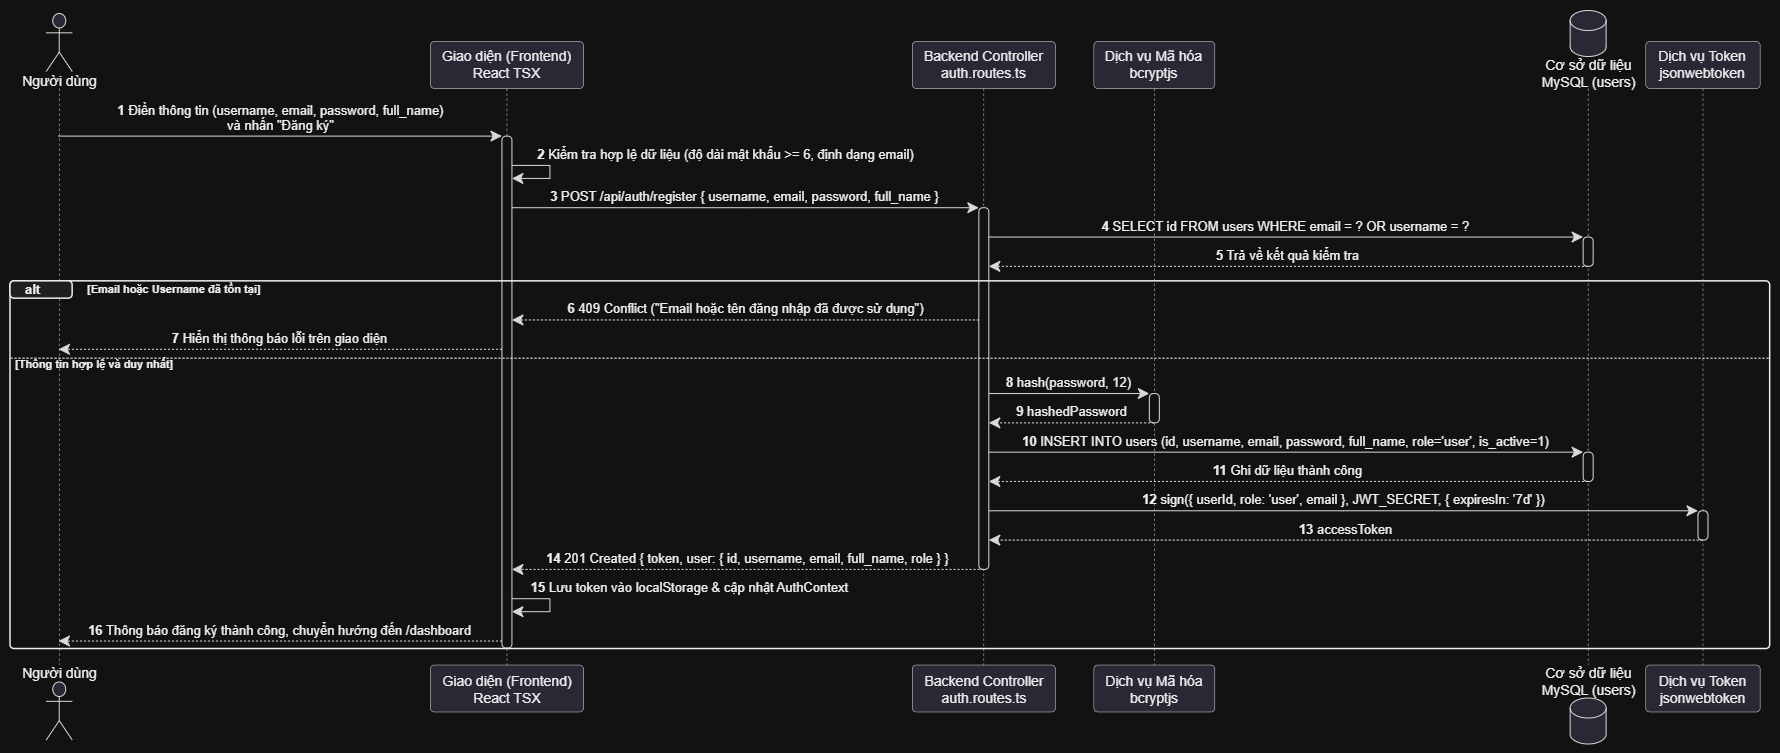
\includegraphics[width=0.94\textwidth]{figs/seq_dang_ky.png}
\caption{Sơ đồ tuần tự quy trình Đăng ký tài khoản người dùng mới.}
\label{fig:seq_dang_ky}
\end{figure}

\noindent\textbf{Mô tả:} Hình~\ref{fig:seq_dang_ky} mô tả sơ đồ tuần tự quy trình đăng ký tài khoản mới giữa Người dùng, Giao diện RegisterPage, Bộ điều khiển AuthController, Thư viện BCrypt và Cơ sở dữ liệu MySQL (bảng users). Luồng tương tác bao gồm: nhập dữ liệu, kiểm tra định dạng tại client, gửi yêu cầu POST /api/auth/register, truy vấn kiểm tra trùng lặp email/username, băm mật khẩu và lưu hồ sơ tài khoản mới.

\noindent\textbf{Diễn giải:} Quy trình này thiết lập cơ chế xác thực hai lớp nghiêm ngặt nhằm bảo vệ an toàn thông tin. Kiểm tra Regex phía client giúp người dùng nhận phản hồi tức thời về định dạng hợp lệ. Ở tầng server, thao tác kiểm tra tính duy nhất giúp loại trừ hoàn toàn nguy cơ trùng lặp danh tính, và việc băm mật khẩu bằng BCrypt với salt rounds = 12 đảm bảo dữ liệu đăng nhập không bao giờ bị lưu dưới dạng văn bản thô (plain text), triệt tiêu rủi ro lộ lọt thông tin.

\subsubsection{2. Sơ đồ tuần tự Đăng nhập và Phân quyền người dùng}

Quy trình xác thực đăng nhập và bảo vệ phiên làm việc dựa trên mã chứng thực JSON Web Token (JWT) được thể hiện tại Hình~\ref{fig:seq_dang_nhap}:
\begin{enumerate}[leftmargin=1.6em, itemsep=2pt]
  \item Người dùng nhập email và mật khẩu tại trang đăng nhập, nhấn nút \en{``Đăng nhập''}.
  \item Frontend kiểm tra tính hợp lệ cơ bản của dữ liệu và gửi yêu cầu \code{POST /api/auth/login}.
  \item \code{Auth Controller} truy vấn bảng \code{users} theo địa chỉ email đã cung cấp.
  \item Nếu không tìm thấy tài khoản, trả về mã lỗi \code{HTTP 401 Unauthorized}. Nếu tìm thấy, kiểm tra cờ trạng thái \code{is\_active}: nếu tài khoản đang bị khóa (giá trị 0), hệ thống chặn đăng nhập và trả về thông báo lỗi tài khoản bị vô hiệu hóa.
  \item Nếu tài khoản đang hoạt động, gọi hàm \code{bcrypt.compare()} để so khớp mật khẩu người dùng nhập với chuỗi băm lưu trữ trong CSDL.
  \item Khi xác thực thành công, hệ thống sử dụng bí mật \code{JWT\_SECRET} để ký số tạo mã chứng thực \code{JWT token} có thời hạn 7 ngày, chứa định danh \code{userId} và vai trò \code{role}.
  \item Trả về mã phản hồi \code{HTTP 200 OK} kèm token và thông tin hồ sơ người dùng.
  \item Frontend lưu JWT vào \code{localStorage}, cập nhật trạng thái toàn cục trong \code{AuthContext}.
  \item Dựa trên trường \code{role}, hệ thống tự động phân luồng điều hướng: nếu là Quản trị viên (\code{admin}) chuyển sang bảng điều khiển \code{/admin}; nếu là Khách hàng (\code{user}) chuyển sang trang chủ \code{/dashboard}.
\end{enumerate}

\begin{figure}[H]
\centering
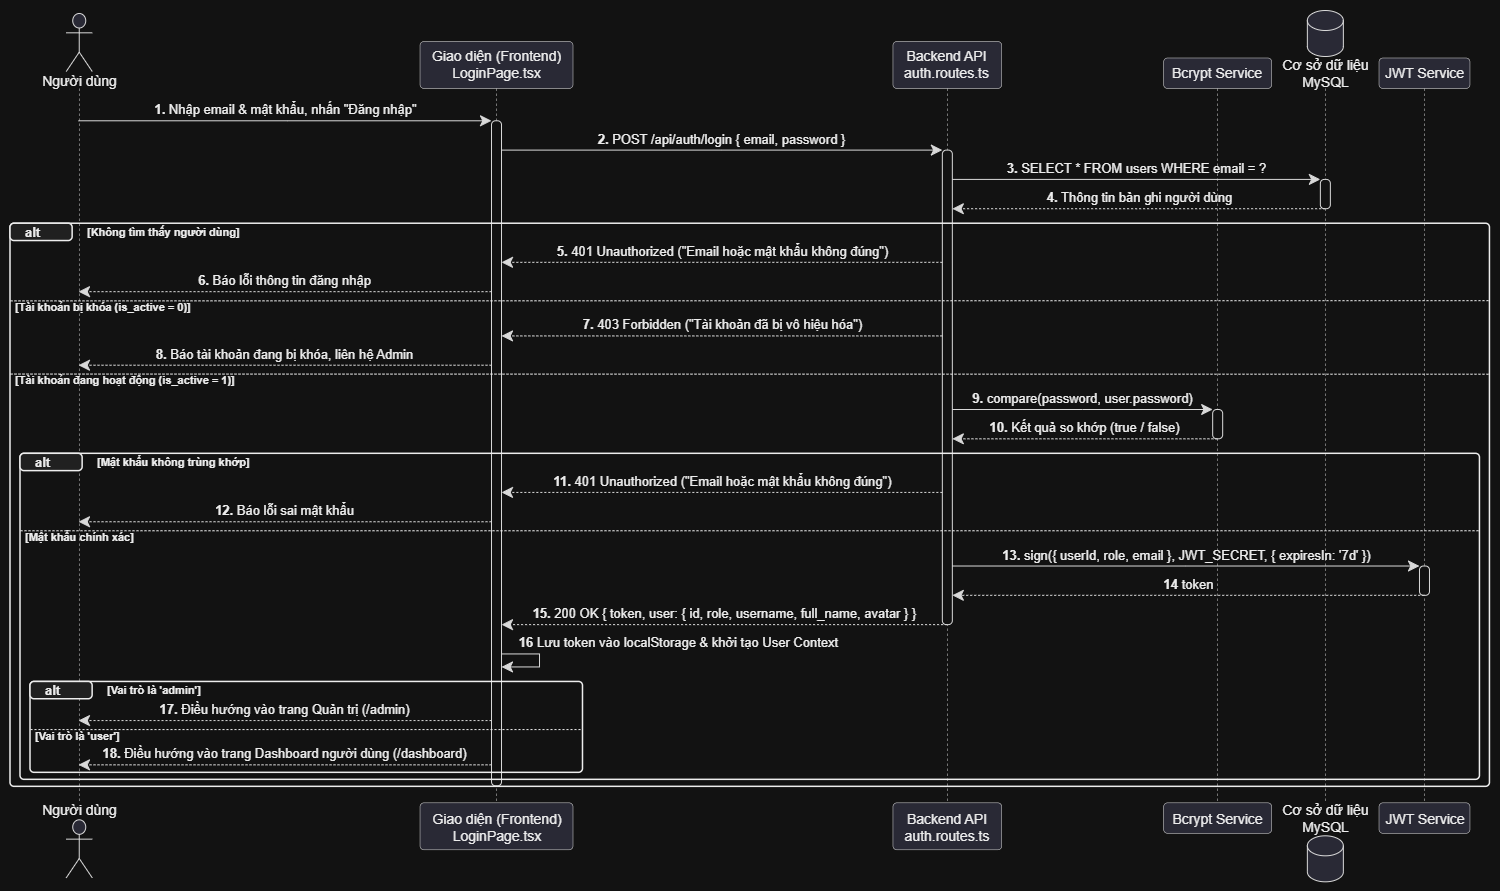
\includegraphics[width=0.96\textwidth]{figs/seq_dang_nhap.png}
\caption{Sơ đồ tuần tự quy trình Đăng nhập và Phân quyền người dùng (JWT).}
\label{fig:seq_dang_nhap}
\end{figure}

\noindent\textbf{Mô tả:} Hình~\ref{fig:seq_dang_nhap} mô tả sơ đồ tuần tự quy trình đăng nhập và phân quyền truy cập gồm các tác tử và đối tượng: Người dùng, LoginPage, AuthController, BCrypt, MySQL (users table) và AuthContext. Các bước thể hiện tuần tự từ khâu gửi thông tin đăng nhập, xác minh sự tồn tại của tài khoản, kiểm tra trạng thái hoạt động (is\_active), so khớp băm mật khẩu, ký tạo JWT token đến lưu trữ phiên làm việc và phân luồng điều hướng theo vai trò.

\noindent\textbf{Diễn giải:} Sơ đồ làm rõ cách thức hệ thống áp dụng giao thức xác thực phi trạng thái (Stateless Authentication) qua JWT. Việc kiểm tra trường is\_active trước khi so sánh mật khẩu giúp ngăn chặn kịp thời các tài khoản đã bị quản trị viên đình chỉ hoạt động. Token được ký bảo mật chứa mã người dùng và quyền hạn (role) cho phép phía Client nhận biết ngay quyền của người dùng để điều hướng chuẩn xác sang giao diện phù hợp (Dashboard cho User hoặc Admin Panel cho Quản trị viên), đồng thời bảo vệ các API nghiệp vụ tiếp theo không bị truy cập trái phép.

\subsubsection{3. Sơ đồ tuần tự Gợi ý món ăn thông minh Hybrid}

Quy trình gợi ý món ăn thông minh là chức năng hạt nhân của hệ thống FoodAI, tích hợp mô hình ngôn ngữ lớn Google Gemini AI cùng cơ chế phòng vệ dự phòng Fallback khi mất mạng (Hình~\ref{fig:seq_goi_y_mon_an}):
\begin{enumerate}[leftmargin=1.6em, itemsep=2pt]
  \item Người dùng nhập danh sách nguyên liệu hoặc chọn nhanh từ các bộ combo gợi ý, nhấn nút \en{``Gợi ý món ăn''}.
  \item Frontend gửi yêu cầu \code{POST /api/recipes/suggest} đính kèm danh sách nguyên liệu và mã Bearer JWT token.
  \item \code{Recipe Controller} xác thực token qua middleware, đồng thời kích hoạt bộ kiểm soát tần suất \en{Rate Limiting} (tối đa 20 yêu cầu/phút) để ngăn chặn hành vi tấn công từ chối dịch vụ.
  \item Hệ thống bất đồng bộ lưu vết danh sách nguyên liệu vào bảng \code{search\_history} phục vụ tính năng tái sử dụng và thống kê quản trị.
  \item \code{Recipe Controller} chuyển tiếp dữ liệu sang mô-đun \code{gemini.service.ts}.
  \item \code{Gemini Service} thiết lập Prompt kỹ thuật cao theo cấu trúc phân vai chuyên gia ẩm thực (\en{AI Chef \& Nutritionist}), kích hoạt chế độ ép kiểu dữ liệu \code{responseMimeType: 'application/json'} và áp dụng nghiêm ngặt quy tắc loại trừ cấm tự bịa thành phần đạm chính (thịt/cá lạ).
  \item Gửi Prompt tới đám mây Google Gemini thông qua thư viện \code{@google/generative-ai}.
\end{enumerate}

Luồng xử lý được rẽ nhánh linh hoạt theo hai kịch bản:
\begin{itemize}[leftmargin=1.6em, itemsep=2pt]
  \item \textbf{Kịch bản chính (Google Gemini phản hồi thành công):}
  \begin{itemize}
    \item Google Gemini trả về chuỗi văn bản JSON chứa danh sách 6 món ăn kèm mẹo nấu và 8 chỉ số dinh dưỡng.
    \item \code{Gemini Service} tiến hành làm sạch ký tự Markdown (\code{```json}), phân tích cú pháp chuỗi JSON, lọc khử trùng lặp và kích hoạt hàm \code{extractPrimaryIngredients} rà soát đạm lạ.
    \item Hệ thống gọi \code{Image Service} để truy vấn kho ảnh Cookpad từ bảng \code{cookpad\_dish\_images}, áp dụng thuật toán chấm điểm \code{scoreRecipeCard} nhằm loại bỏ các hình ảnh bento tạo hình hoặc đồ ăn dặm.
    \item Gán đường dẫn ảnh thực tế chất lượng cao độc nhất cho từng món gợi ý, đảm bảo không có hai món nào bị trùng ảnh trong cùng một phiên tìm kiếm.
    \item Trả về danh sách 6 món ăn hoàn chỉnh với cờ nguồn \code{source = 'ai'}.
  \end{itemize}
  \item \textbf{Kịch bản dự phòng (Sự cố mạng, Timeout hoặc vượt Quota):}
  \begin{itemize}
    \item Khi xảy ra lỗi kết nối bên thứ ba, khối \code{catch} bắt ngoại lệ và kích hoạt ngay hàm dự phòng \code{suggestRecipesFromDatabase()}.
    \item Truy vấn trực tiếp từ bảng \code{recipes} trong CSDL MySQL theo giải thuật so khớp Heuristic với ma trận nguyên liệu đồng nghĩa và ranh giới từ nguyên vẹn.
    \item Trả về danh sách món ăn từ kho Cookpad nội bộ với cờ nguồn \code{source = 'fallback'} mà không gây gián đoạn trải nghiệm người dùng.
  \end{itemize}
\end{itemize}

Frontend tiếp nhận kết quả phản hồi \code{HTTP 200 OK} và kết xuất danh sách Recipe Card trực quan ra màn hình.

\begin{figure}[H]
\centering
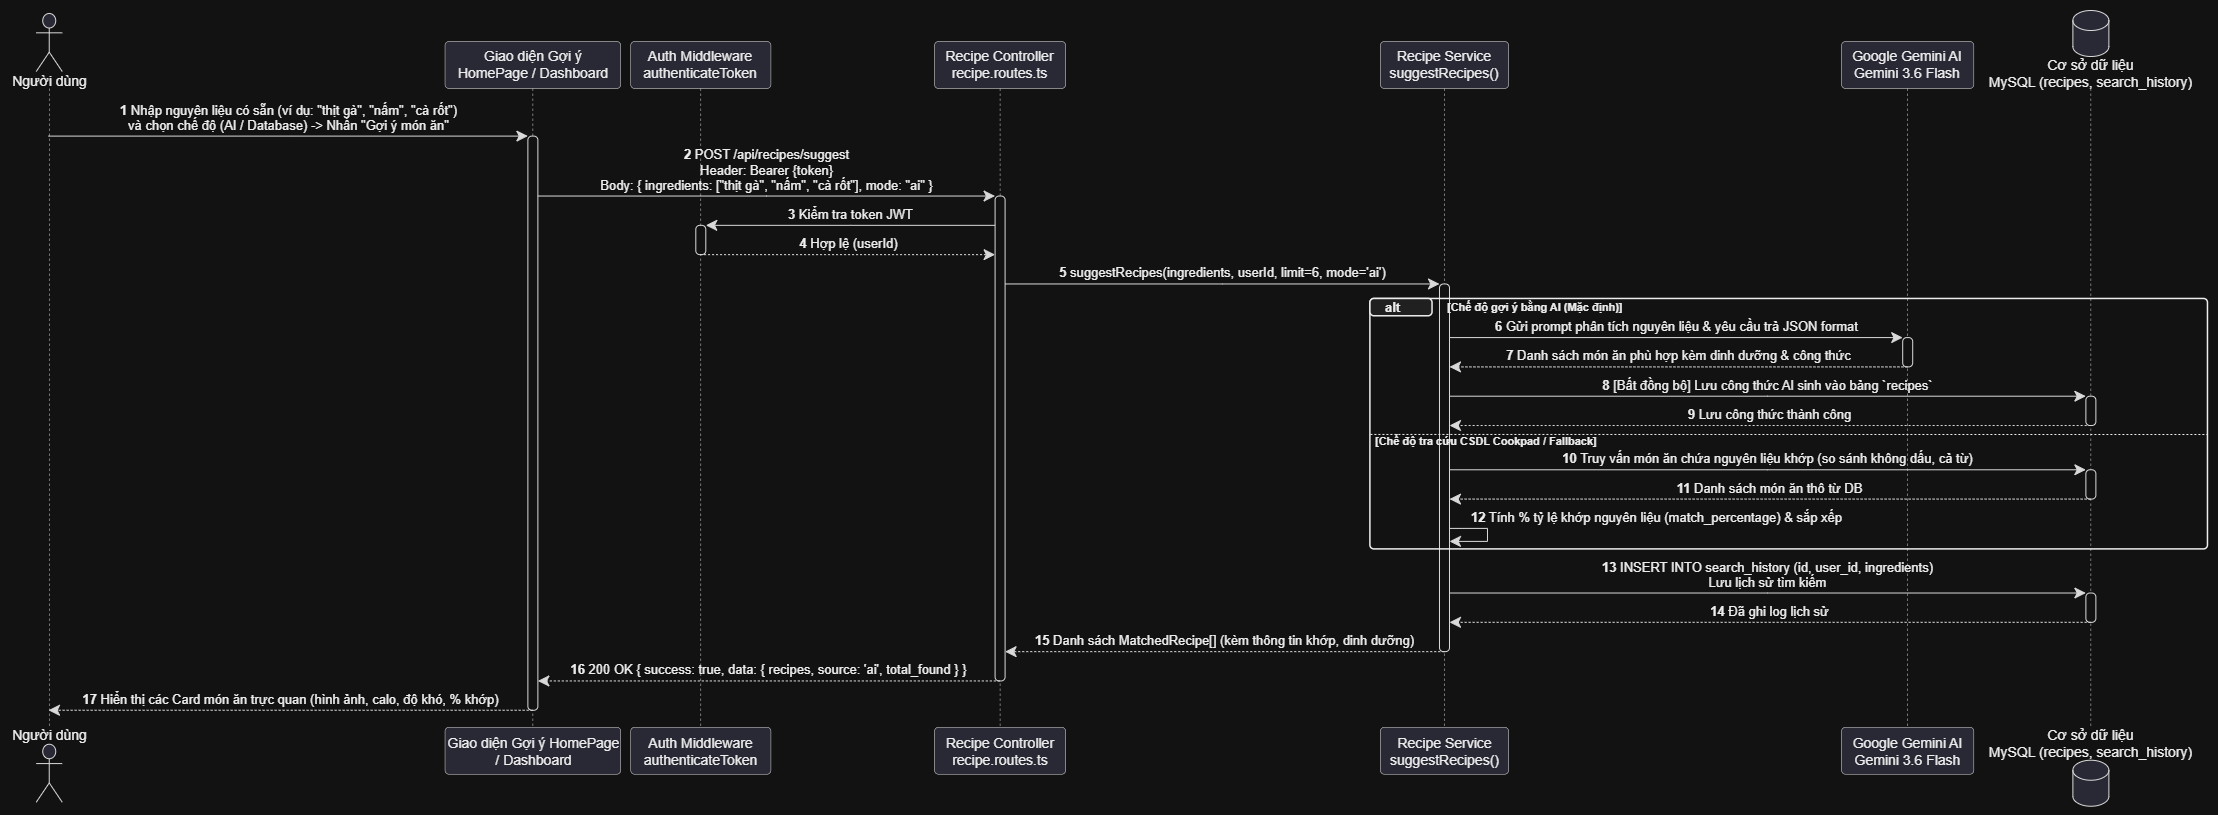
\includegraphics[width=\textwidth]{figs/seq_goi_y_mon_an.png}
\caption{Sơ đồ tuần tự quy trình Gợi ý món ăn thông minh Hybrid.}
\label{fig:seq_goi_y_mon_an}
\end{figure}

\noindent\textbf{Mô tả:} Hình~\ref{fig:seq_goi_y_mon_an} mô tả sơ đồ tuần tự quy trình gợi ý món ăn thông minh theo kiến trúc kết hợp (Hybrid) giữa Người dùng, Dashboard UI, RecipeController, GeminiService, ImageService và CSDL MySQL. Sơ đồ minh họa rành mạch hai nhánh xử lý: (1) Nhánh chính với Google Gemini AI khi có kết nối mạng và API Key hợp lệ, trải qua các bước làm sạch JSON, hậu kiểm loại trừ đạm lạ và gán ảnh Cookpad; (2) Nhánh dự phòng Fallback tự động kích hoạt khi AI gặp sự cố để truy xuất trực tiếp từ kho món ăn Cookpad MySQL nội bộ.

\noindent\textbf{Diễn giải:} Sơ đồ này chứng minh tính chịu lỗi (Fault-Tolerant) và độ sẵn sàng cao của hệ thống FoodAI. Việc kết hợp AI tạo sinh với quy tắc lọc ngữ nghĩa tiếng Việt nghiêm ngặt giải quyết triệt để vấn đề ảo giác nguyên liệu thịt cá mà các mô hình ngôn ngữ lớn thường gặp phải. Khi xảy ra sự cố mạng bên ngoài hoặc vượt định ngạch API, cơ chế Fallback nội bộ phản hồi ngay lập tức trong thời gian dưới 300ms, đảm bảo người dùng luôn nhận được gợi ý món ăn có liên quan mà trải nghiệm không bao giờ bị gián đoạn.

\subsubsection{4. Sơ đồ tuần tự Xem chi tiết công thức nấu và Phân tích dinh dưỡng}

Quy trình xem chi tiết công thức và thông tin vi chất hỗ trợ người dùng có được bức tranh toàn diện trước khi bắt tay vào chế biến (Hình~\ref{fig:seq_xem_chi_tiet_dinh_duong}):
\begin{enumerate}[leftmargin=1.6em, itemsep=2pt]
  \item Người dùng nhấn vào thẻ món ăn hoặc nút \en{``Xem chi tiết''} trên giao diện trang chủ.
  \item Frontend gửi yêu cầu trích xuất chi tiết công thức hoặc kích hoạt Modal 3 Tab tích hợp sẵn từ dữ liệu gợi ý.
  \item Nếu là món ăn chưa có đầy đủ hướng dẫn từng bước, hệ thống gửi yêu cầu \code{POST /api/recipes/ai-recipe-detail} kèm tên món ăn lên Backend.
  \item \code{Gemini Service} sinh bản phân tích chuyên sâu gồm: định lượng chính xác từng nguyên liệu (gam/ml), danh sách các bước nấu nướng tuần tự kèm thời gian chế biến, và bảng 8 chỉ số dinh dưỡng định lượng (năng lượng calo, protein, carbs, chất béo, chất xơ, vitamin C, canxi, sắt).
  \item Backend trả về đối tượng chi tiết cấu trúc JSON chuẩn về cho Frontend.
  \item Frontend hiển thị cửa sổ Modal tương tác với 3 phân hệ rành mạch: Tab 1 --- Định lượng nguyên liệu (đánh dấu xanh các nguyên liệu đã có); Tab 2 --- Hướng dẫn nấu ăn 4--6 bước rõ ràng; Tab 3 --- Bảng vi chất dinh dưỡng khoa học.
\end{enumerate}

\begin{figure}[H]
\centering
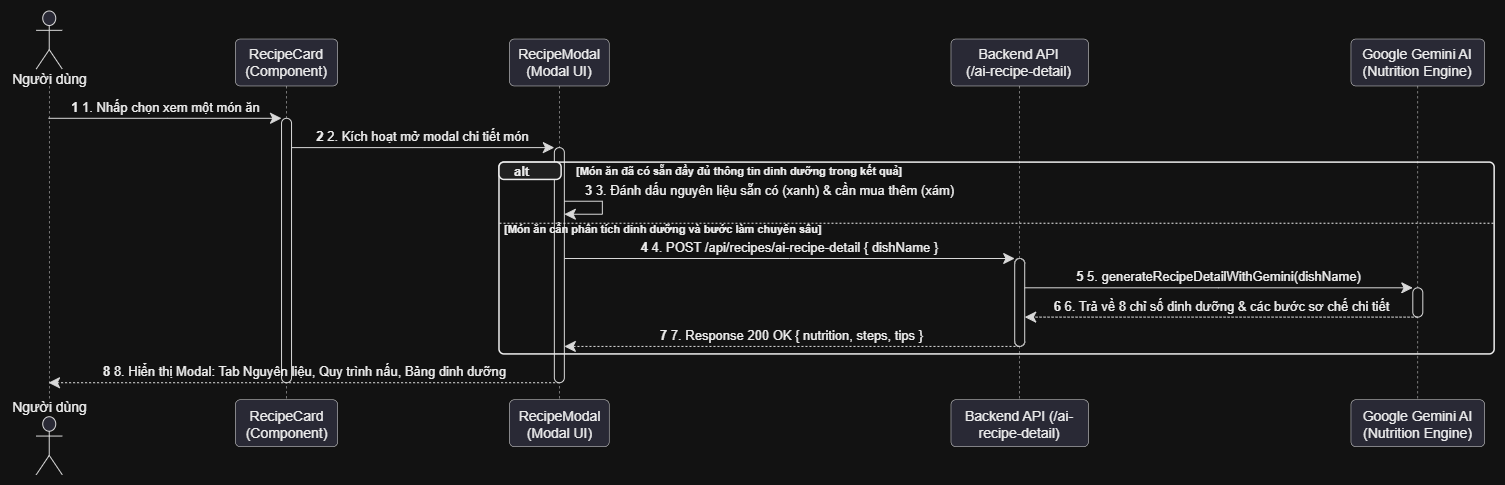
\includegraphics[width=0.94\textwidth]{figs/seq_xem_chi_tiet_dinh_duong.png}
\caption{Sơ đồ tuần tự quy trình Xem chi tiết công thức nấu và Phân tích dinh dưỡng.}
\label{fig:seq_xem_chi_tiet_dinh_duong}
\end{figure}

\noindent\textbf{Mô tả:} Hình~\ref{fig:seq_xem_chi_tiet_dinh_duong} mô tả sơ đồ tuần tự quy trình hiển thị chi tiết công thức và phân tích dinh dưỡng giữa Người dùng, RecipeCard/Modal, RecipeController, GeminiService và cơ sở dữ liệu. Luồng thực hiện gồm: kích hoạt xem chi tiết từ thẻ món, kiểm tra tính đầy đủ của dữ liệu công thức, gọi mô-đun AI làm giàu thêm thông tin nếu cần thiết, và kết xuất dữ liệu phân chia theo 3 tab chuyên biệt trên giao diện Modal.

\noindent\textbf{Diễn giải:} Quy trình này làm nổi bật năng lực chuyên gia ẩm thực (AI Chef) và chuyên gia dinh dưỡng của hệ thống. Thay vì chỉ cung cấp công thức nấu đơn thuần như các trang mạng truyền thống, việc tích hợp bảng 8 chỉ số vi chất dinh dưỡng (calo, protein, carbs, fat, xơ, vitamin C, canxi, sắt) giúp người dùng quản lý khẩu phần ăn khoa học. Thiết kế giao diện 3 Tab phân tách rõ nguyên liệu có sẵn và nguyên liệu cần chuẩn bị thêm, giúp người dùng dễ dàng lập kế hoạch nấu nướng.

\subsubsection{5. Sơ đồ tuần tự Quản lý và Lưu món ăn yêu thích}

Quy trình quản lý sổ tay ẩm thực cá nhân cho phép người dùng lưu lại những công thức yêu thích để nấu lại sau này (Hình~\ref{fig:seq_quan_ly_yeu_thich}):
\begin{enumerate}[leftmargin=1.6em, itemsep=2pt]
  \item Người dùng nhấn vào biểu tượng Trái tim trên Card món ăn hoặc bên trong Modal chi tiết.
  \item Giao diện gửi yêu cầu \code{POST /api/recipes/favorites} mang theo toàn bộ đối tượng dữ liệu món ăn dạng JSON cùng mã chứng thực Bearer JWT token.
  \item \code{Recipe Controller} giải mã token để trích xuất \code{userId} và kiểm tra tính hợp lệ của gói tin.
  \item Hệ thống thực thi câu lệnh \code{SELECT} trên bảng \code{favorite\_recipes} để kiểm tra xem món ăn này đã được người dùng lưu trước đó hay chưa (dựa theo \code{recipe\_id} hoặc tên món ăn).
  \item Nếu món ăn đã tồn tại, phản hồi mã lỗi \code{HTTP 409 Conflict} để tránh lưu trùng lặp.
  \item Nếu chưa tồn tại, hệ thống khởi tạo khóa chính UUID v4 và thực thi lệnh \code{INSERT INTO favorite\_recipes} lưu trữ toàn bộ dữ liệu công thức vào trường \code{recipe\_data}.
  \item Cơ sở dữ liệu xác nhận ghi dữ liệu thành công, phản hồi mã trạng thái \code{HTTP 200 OK}.
  \item Frontend chuyển trạng thái icon trái tim sang màu đỏ kích hoạt \en{(Active State)}, đồng thời hiển thị thông báo Toast xác nhận: \en{``Đã thêm vào danh sách yêu thích''}.
\end{enumerate}

\begin{figure}[H]
\centering
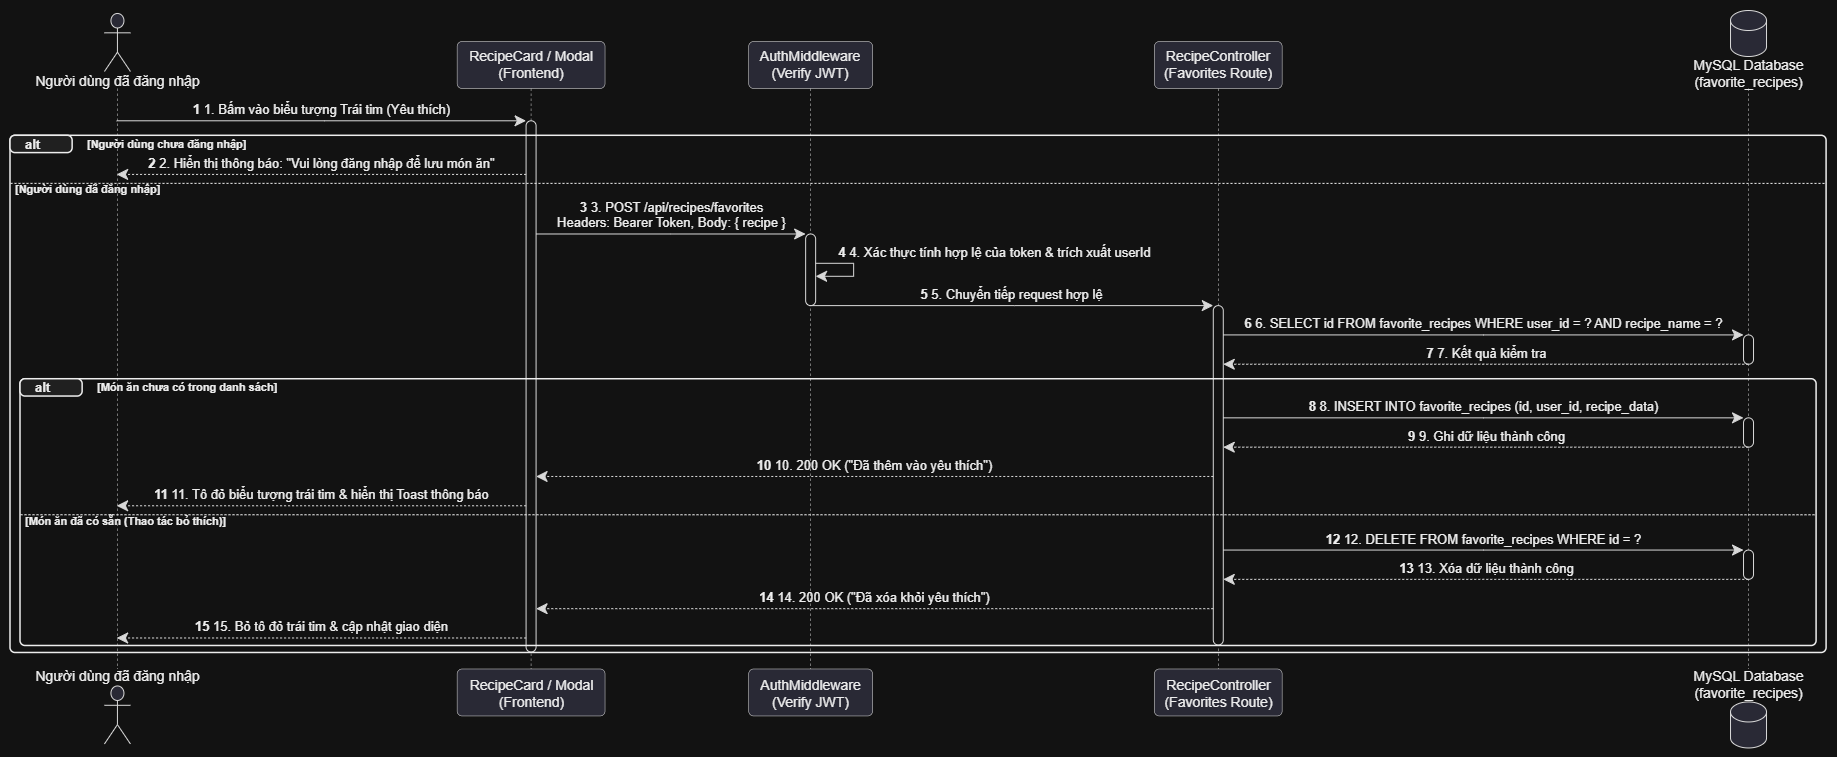
\includegraphics[width=0.94\textwidth]{figs/seq_quan_ly_yeu_thich.png}
\caption{Sơ đồ tuần tự quy trình Quản lý và Lưu món ăn yêu thích.}
\label{fig:seq_quan_ly_yeu_thich}
\end{figure}

\noindent\textbf{Mô tả:} Hình~\ref{fig:seq_quan_ly_yeu_thich} mô tả sơ đồ tuần tự lưu trữ món ăn yêu thích của người dùng, liên kết tương tác giữa Người dùng, Nút biểu tượng Trái tim, RecipeController, Middleware JWT và bảng favorite\_recipes trong MySQL. Trình tự bao gồm: nhấn icon yêu thích, kiểm tra phiên đăng nhập bằng JWT, kiểm tra trùng lặp bản ghi trong cơ sở dữ liệu, chèn bản ghi JSON công thức mới và cập nhật trạng thái hiển thị của icon trên giao diện.

\noindent\textbf{Diễn giải:} Sơ đồ thể hiện kỹ thuật quản lý dữ liệu cá nhân hóa an toàn. Việc liên kết món ăn yêu thích với định danh userId lấy trực tiếp từ JWT ngăn chặn hoàn toàn việc người dùng can thiệp vào bộ sưu tập của người khác. Cơ chế kiểm tra trùng lặp trước khi thực hiện lệnh INSERT giúp cơ sở dữ liệu duy trì tính toàn vẹn, tránh lãng phí dung lượng lưu trữ và ngăn ngừa xung đột dữ liệu khi người dùng vô tình bấm nhiều lần liên tiếp.

\subsubsection{6. Sơ đồ tuần tự Quản trị tài khoản người dùng}

Phân hệ quản trị dành riêng cho Quản trị viên (\code{Admin}) để quản lý vòng đời tài khoản người dùng và giám sát hệ thống (Hình~\ref{fig:seq_quan_tri_nguoi_dung}):
\begin{enumerate}[leftmargin=1.6em, itemsep=2pt]
  \item Quản trị viên đăng nhập với tài khoản Admin và truy cập vào đường dẫn quản trị người dùng \code{/admin/users}.
  \item Frontend gửi yêu cầu \code{GET /api/admin/users} có đính kèm Bearer token tới máy chủ.
  \item Middleware \code{authenticateToken} và bộ lọc phân quyền \code{requireAdmin} kiểm tra tính hợp lệ của token và xác minh vai trò \code{role === 'admin'}. Nếu không phải admin, hệ thống từ chối truy cập với mã lỗi \code{HTTP 403 Forbidden}.
  \item Khi xác thực thành công, \code{Admin Controller} thực thi truy vấn lấy danh sách toàn bộ người dùng có phân trang (10 bản ghi/trang), kèm thông tin tổng hợp số lượt tìm kiếm và số món ăn đã lưu.
  \item CSDL MySQL trả về tập dữ liệu, máy chủ gửi phản hồi \code{HTTP 200 OK} về Frontend để kết xuất bảng dữ liệu trực quan.
  \item Khi Quản trị viên thực hiện thao tác thay đổi trạng thái (Kích hoạt/Vô hiệu hóa tài khoản) hoặc Đặt lại mật khẩu:
  \begin{itemize}
    \item Frontend gửi yêu cầu \code{PUT /api/admin/users/:id/status} hoặc \code{PUT /api/admin/users/:id/reset-password}.
    \item Hệ thống kiểm tra quy tắc an toàn cốt lõi: Quản trị viên tuyệt đối không thể tự khóa hoặc tự xóa tài khoản của chính mình.
    \item \code{Admin Controller} thực thi cập nhật bản ghi trong bảng \code{users} và phản hồi thông báo thành công.
    \item Frontend cập nhật trạng thái bảng dữ liệu theo thời gian thực (Real-time UI Update) và hiển thị thông báo Toast.
  \end{itemize}
\end{enumerate}

\begin{figure}[H]
\centering
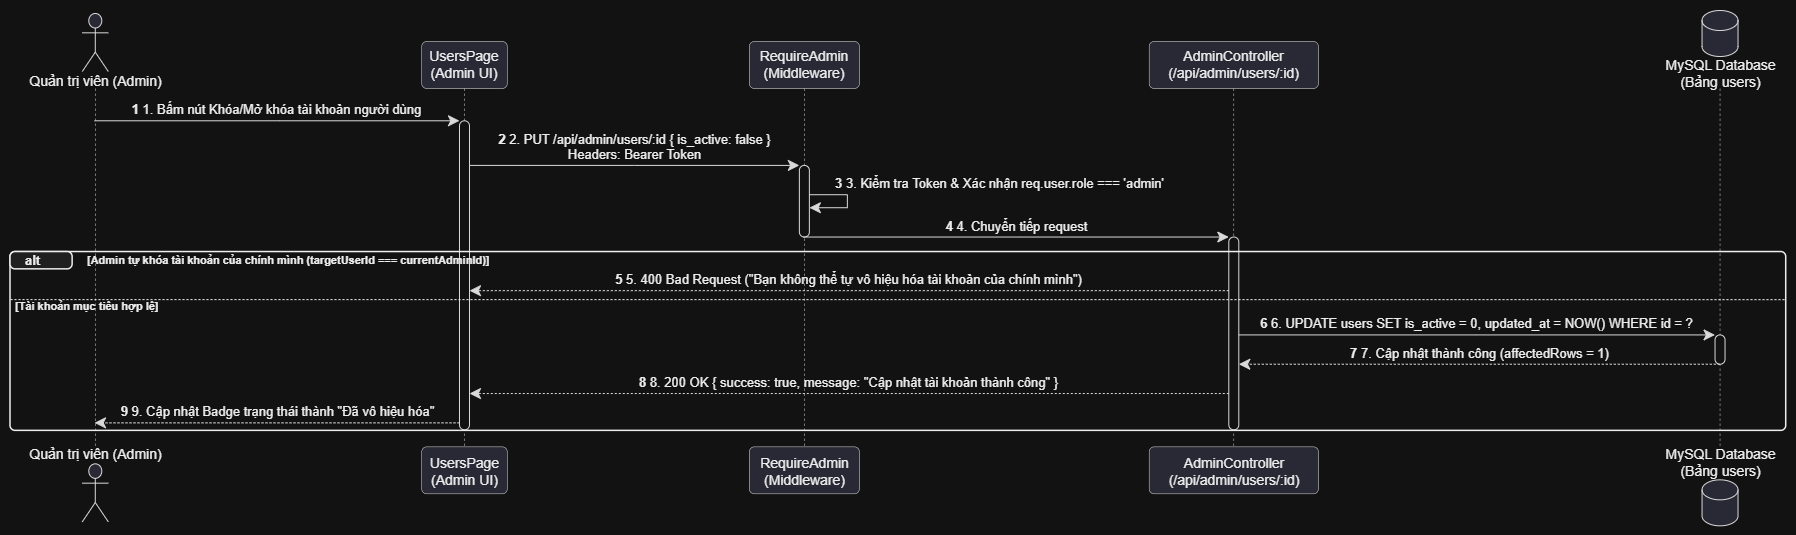
\includegraphics[width=0.94\textwidth]{figs/seq_quan_tri_nguoi_dung.png}
\caption{Sơ đồ tuần tự quy trình Quản trị tài khoản người dùng.}
\label{fig:seq_quan_tri_nguoi_dung}
\end{figure}

\noindent\textbf{Mô tả:} Hình~\ref{fig:seq_quan_tri_nguoi_dung} mô tả sơ đồ tuần tự các thao tác quản trị tài khoản người dùng, bao gồm: Quản trị viên, Trang AdminUsersPage, Bộ kiểm soát phân quyền requireAdmin Middleware, AdminController và bảng users trong CSDL MySQL. Sơ đồ biểu diễn hai luồng chính: tải danh sách tài khoản phân trang kèm số liệu thống kê và thực hiện cập nhật trạng thái kích hoạt/khóa tài khoản hoặc đặt lại mật khẩu.

\noindent\textbf{Diễn giải:} Sơ đồ làm rõ tầng phòng thủ bảo mật cấp cao nhất của hệ thống. Bộ lọc requireAdmin chặn đứng từ cửa ngõ các yêu cầu giả mạo từ người dùng thông thường bằng mã lỗi HTTP 403 Forbidden. Điểm đặc biệt quan trọng trong nghiệp vụ là cơ chế kiểm tra an toàn tại server: ngăn chặn tuyệt đối tình huống Quản trị viên tự khóa tài khoản của chính mình, đảm bảo hệ thống luôn luôn có ít nhất một tài khoản Admin đang hoạt động để duy trì quyền điều hành.

\section{Thiết kế kiến trúc hệ thống}

Hệ thống được thiết kế theo mô hình kiến trúc ba tầng \en{(Three-Tier Architecture)} hiện đại, đảm bảo tính mô-đun hóa, bảo mật và khả năng mở rộng dễ dàng (Hình~\ref{fig:kientruc_hethong}).

\begin{figure}[H]
\centering
\resizebox{\textwidth}{!}{%
\begin{tikzpicture}[node distance=10mm and 12mm]
  % Tầng Client
  \node[startstop, fill=lightnavy, draw=daunavy] (client) {\textbf{TẦNG GIAO DIỆN (CLIENT LAYER)}\\React 18 + TypeScript + Vite + Tailwind CSS\\(User Dashboard \& Admin Dashboard)};

  % Tầng Server
  \node[process, fill=white, draw=daumaroon, below=12mm of client] (server) {\textbf{TẦNG ỨNG DỤNG (SERVER LAYER)}\\Node.js + Express RESTful API\\Auth Middleware (JWT) $\cdot$ Rate Limiter $\cdot$ CORS};

  % Khối dịch vụ bên trong Server
  \node[clsbox, below left=10mm and -5mm of server] (ai_svc) {Gemini Service\\(AI Chef \& Nutritionist)};
  \node[clsbox, below=10mm of server] (recipe_svc) {Recipe Service\\(Heuristic Matching)};
  \node[clsbox, below right=10mm and -5mm of server] (img_svc) {Image Service\\(Multi-source Retrieval)};

  % Tầng Dữ liệu & AI bên ngoài
  \node[objbox, below=14mm of recipe_svc] (db) {\textbf{CƠ SỞ DỮ LIỆU}\\MySQL 8.0 / SQLite\\(Users, Recipes, Cookpad Images, Favorites, History)};

  \node[membox, left=10mm of db] (gemini_ext) {\textbf{Google Gemini API}\\(LLM Engine)};
  \node[membox, right=10mm of db] (pexels_ext) {\textbf{Pexels \& Cookpad}\\(Image Sources)};

  % Kết nối
  \draw[flowarr] (client) -- node[right, font=\tiny]{HTTPS / JSON} (server);
  \draw[flowarr] (server) -- (ai_svc);
  \draw[flowarr] (server) -- (recipe_svc);
  \draw[flowarr] (server) -- (img_svc);
  \draw[flowarr] (ai_svc) -- (gemini_ext);
  \draw[flowarr] (recipe_svc) -- (db);
  \draw[flowarr] (img_svc) -- (pexels_ext);
  \draw[flowarr] (img_svc) -- (db);
\end{tikzpicture}}
\caption{Sơ đồ kiến trúc phân tầng tổng thể của hệ thống FoodAI.}
\label{fig:kientruc_hethong}
\end{figure}

\noindent\textbf{Mô tả:} Hình~\ref{fig:kientruc_hethong} mô tả kiến trúc phân tầng tổng thể của hệ thống FoodAI theo mô hình 3 tầng (Three-Tier Architecture), bao gồm: (1) Tầng giao diện Client Layer (React 18, TypeScript, Vite, Tailwind CSS); (2) Tầng ứng dụng Server Layer (Node.js, Express RESTful API với các khối Auth Middleware, Rate Limiter, Gemini Service, Recipe Service, Image Service); và (3) Tầng dữ liệu \& dịch vụ bên ngoài (CSDL MySQL 8.0, Google Gemini API, Pexels API và kho ảnh Cookpad).

\noindent\textbf{Diễn giải:} Sơ đồ thể hiện tính phân tách trách nhiệm (Separation of Concerns) cao giữa các tầng. Mọi yêu cầu từ Client đều phải thông qua giao thức HTTPS có kiểm soát bởi Middleware xác thực và giới hạn tần suất (Rate Limiter) trước khi chạm tới các dịch vụ nghiệp vụ. Việc bóc tách các Service độc lập (Gemini Service cho AI, Recipe Service cho giải thuật so khớp, Image Service cho truy xuất ảnh) giúp mã nguồn đạt độ gắn kết cao, giảm thiểu phụ thuộc lỏng lẻo, tạo điều kiện thuận lợi cho việc kiểm thử đơn vị, bảo trì và mở rộng tính năng mà không gây ảnh hưởng tới toàn bộ hệ thống.

\section{Thiết kế cơ sở dữ liệu}

Cơ sở dữ liệu quan hệ của hệ thống được thiết kế chuẩn hóa để lưu trữ thông tin người dùng, công thức ẩm thực, hình ảnh cào từ Cookpad và dữ liệu tương tác (Bảng~\ref{tab:schema_users} và Bảng~\ref{tab:schema_recipes}).

\begin{table}[H]
\centering
\caption{Lược đồ cấu trúc bảng người dùng (\code{users}).}
\label{tab:schema_users}
\begin{tabularx}{\textwidth}{@{}>{\bfseries\color{daunavy}}p{2.6cm} >{\color{daumaroon}}p{2.8cm} >{\raggedright\arraybackslash}X@{}}
\toprule
\rowcolor{gray100}\bfseries\color{daunavy}Tên cột & \bfseries\color{daumaroon}Kiểu dữ liệu & \bfseries\color{daunavy}Ràng buộc \& Ý nghĩa \\
\midrule
id          & VARCHAR(36)  & Khóa chính (UUID v4) \\
username    & VARCHAR(50)  & Tên đăng nhập duy nhất (UNIQUE, NOT NULL) \\
email       & VARCHAR(100) & Địa chỉ email duy nhất (UNIQUE, NOT NULL) \\
password    & VARCHAR(255) & Mật khẩu đã băm (Bcrypt hash) \\
full\_name  & VARCHAR(100) & Họ và tên hiển thị \\
role        & VARCHAR(10)  & Vai trò tài khoản (\code{'user'} hoặc \code{'admin'}) \\
is\_active  & TINYINT(1)   & Trạng thái kích hoạt tài khoản (1: Hoạt động, 0: Khóa) \\
created\_at & DATETIME     & Thời điểm tạo tài khoản \\
\bottomrule
\end{tabularx}
\end{table}

\noindent\textbf{Mô tả:} Bảng~\ref{tab:schema_users} mô tả chi tiết lược đồ cấu trúc của bảng \code{users} gồm 8 trường dữ liệu: id (khóa chính UUID), username (tên đăng nhập duy nhất), email (địa chỉ thư điện tử duy nhất), password (chuỗi băm BCrypt 255 ký tự), full\_name (họ tên hiển thị), role (vai trò người dùng), is\_active (cờ trạng thái kích hoạt) và created\_at (mốc thời gian tạo tài khoản).

\noindent\textbf{Diễn giải:} Thiết kế bảng đáp ứng chuẩn dạng chuẩn 3 (3NF) trong cơ sở dữ liệu quan hệ. Ràng buộc UNIQUE trên hai trường username và email ngăn chặn tuyệt đối tình trạng đăng ký trùng lặp tài khoản. Việc lưu trữ mật khẩu bằng chuỗi băm BCrypt 255 ký tự đảm bảo an toàn tối đa theo các tiêu chuẩn an ninh mạng hiện đại. Trường cờ is\_active cho phép quản trị viên có thể vô hiệu hóa quyền truy cập của tài khoản vi phạm chính sách một cách linh hoạt mà vẫn bảo toàn toàn bộ dữ liệu lịch sử tìm kiếm và món ăn yêu thích liên kết.

\begin{table}[H]
\centering
\caption{Lược đồ cấu trúc bảng món ăn nội bộ (\code{recipes}).}
\label{tab:schema_recipes}
\begin{tabularx}{\textwidth}{@{}>{\bfseries\color{daunavy}}p{2.8cm} >{\color{daumaroon}}p{2.8cm} >{\raggedright\arraybackslash}X@{}}
\toprule
\rowcolor{gray100}\bfseries\color{daunavy}Tên cột & \bfseries\color{daumaroon}Kiểu dữ liệu & \bfseries\color{daunavy}Ràng buộc \& Ý nghĩa \\
\midrule
id            & VARCHAR(36)  & Khóa chính món ăn \\
name          & VARCHAR(255) & Tên món ăn tiếng Việt (INDEX) \\
description   & TEXT         & Mô tả vắn tắt về hương vị \\
image\_url    & VARCHAR(1000)& Đường dẫn ảnh món ăn thực tế \\
cooking\_time & INT          & Thời gian chế biến (phút) \\
difficulty    & VARCHAR(20)  & Độ khó (\code{'Dễ'}, \code{'Trung bình'}, \code{'Khó'}) \\
category      & VARCHAR(50)  & Danh mục (\code{'Món xào'}, \code{'Súp/Canh'}, \dots) \\
author\_name  & VARCHAR(100) & Tác giả chia sẻ công thức trên Cookpad \\
\bottomrule
\end{tabularx}
\end{table}

\noindent\textbf{Mô tả:} Bảng~\ref{tab:schema_recipes} mô tả cấu trúc bảng lưu trữ món ăn \code{recipes} với 8 thuộc tính nòng cốt: id (khóa chính), name (tên món ăn tiếng Việt có đánh chỉ mục INDEX), description (mô tả hương vị), image\_url (đường dẫn hình ảnh CDN), cooking\_time (thời gian nấu ước tính tính theo phút), difficulty (độ khó chế biến), category (danh mục phân loại) và author\_name (tác giả chia sẻ công thức).

\noindent\textbf{Diễn giải:} Bảng \code{recipes} đóng vai trò là cơ sở tri thức ẩm thực nội bộ (Internal Knowledge Base) của hệ thống. Việc đánh chỉ mục INDEX trên trường tên món ăn \code{name} giúp tối ưu hóa đáng kể tốc độ tìm kiếm văn bản và so khớp Heuristic khi hệ thống hoạt động ở chế độ Fallback, giảm thời gian phản hồi từ CSDL xuống dưới mức 50ms. Các trường định lượng như thời gian nấu và mức độ khó cung cấp siêu dữ liệu đầy đủ để giao diện người dùng hiển thị thẻ món ăn trực quan và hỗ trợ bộ lọc đa chiều.

Ngoài ra, hệ thống lưu trữ ảnh trích xuất trong bảng \code{cookpad\_dish\_images}, lưu trữ lịch sử người dùng trong \code{search\_history} và lưu công thức yêu thích dạng JSON chi tiết trong \code{favorite\_recipes}.

\section{Thiết kế thuật toán gợi ý và Xử lý ảnh thông minh}

\subsection{Luồng thực thi gợi ý món ăn thông minh}

Quy trình gợi ý món ăn kết hợp AI và Fallback được mô tả chi tiết tại Hình~\ref{fig:flow_suggest}.

\begin{figure}[H]
\centering
\resizebox{0.82\textwidth}{!}{%
\begin{tikzpicture}[node distance=10mm]
  \node[startstop] (start) {Bắt đầu: Tiếp nhận danh sách nguyên liệu $U$};
  \node[decision, below=8mm of start] (check_key) {Cấu hình Gemini API hợp lệ?};
  \node[process, below left=10mm and 2mm of check_key] (call_ai) {Gọi Google Gemini AI\\với Prompt ràng buộc};
  \node[decision, below=8mm of call_ai] (check_ai) {AI phản hồi \&\\Parse JSON thành công?};
  \node[process, below=8mm of check_ai] (post_filter) {Hậu kiểm: Khử trùng lặp\\và lọc vi phạm thịt cá};
  \node[process, right=20mm of check_ai] (fallback_db) {Kích hoạt chế độ Fallback:\\Tra cứu kho Cookpad MySQL};
  \node[process, below=8mm of post_filter] (attach_img) {Truy xuất \& Gán hình ảnh độc nhất\\từ Cookpad / Pexels / HD Bank};
  \node[startstop, below=8mm of attach_img] (finish) {Trả về danh sách 4--6 món ăn kèm\\công thức, dinh dưỡng và ảnh cho người dùng};

  \draw[flowarr] (start) -- (check_key);
  \draw[flowarr] (check_key) -| node[above, font=\footnotesize]{Có} (call_ai);
  \draw[flowarr] (check_key) -| node[above, font=\footnotesize]{Không} (fallback_db);
  \draw[flowarr] (call_ai) -- (check_ai);
  \draw[flowarr] (check_ai) -- node[right, font=\footnotesize]{Thành công} (post_filter);
  \draw[flowarr] (check_ai) -- node[above, font=\footnotesize]{Lỗi / Timeout} (fallback_db);
  \draw[flowarr] (fallback_db) |- (attach_img);
  \draw[flowarr] (post_filter) -- (attach_img);
  \draw[flowarr] (attach_img) -- (finish);
\end{tikzpicture}}
\caption{Sơ đồ khối luồng xử lý gợi ý món ăn thông minh (Hybrid Flowchart).}
\label{fig:flow_suggest}
\end{figure}

\noindent\textbf{Mô tả:} Hình~\ref{fig:flow_suggest} mô tả sơ đồ lưu đồ (Flowchart) tiến trình xử lý gợi ý món ăn, thể hiện các khối quyết định rẽ nhánh logic từ lúc tiếp nhận danh sách nguyên liệu đầu vào, kiểm tra điều kiện khả dụng của API Key, gọi mô hình Gemini AI, kiểm tra tính hợp lệ của gói tin JSON, tiến hành lọc khử vi phạm nguyên liệu, cơ chế kích hoạt nhánh Fallback cơ sở dữ liệu khi phát sinh lỗi, đến công đoạn gắn hình ảnh và trả về kết quả cuối cùng.

\noindent\textbf{Diễn giải:} Sơ đồ khối giải thích nguyên nhân hệ thống duy trì được tính ổn định và tính chính xác cao. Nhánh xử lý AI được kiểm soát chặt chẽ bởi hai chốt chặn: khối kiểm tra cú pháp JSON đảm bảo cấu trúc dữ liệu không bị gãy vỡ, và khối hậu kiểm ngữ nghĩa loại bỏ ngay các món ăn tự bịa thịt cá vi phạm ràng buộc nguyên liệu đầu vào. Nhánh rẽ Fallback sang kho Cookpad MySQL giải thích vì sao khi mất kết nối mạng hay hết quota Gemini, hệ thống vẫn trả về được các món ăn truyền thống chuẩn vị và có sẵn ảnh chất lượng cao mà không hiển thị màn hình trắng hay báo lỗi khó chịu cho người dùng.

\subsection{Giải thuật gợi ý món ăn theo kiến trúc Database-First RAG (Mã giả)}

Giải thuật gợi ý món ăn áp dụng kỹ thuật RAG định hướng CSDL (\en{Database-First Retrieval-Augmented Generation})~\cite{Lewis2020RAG} kết hợp làm giàu dữ liệu tự động bằng Google Gemini AI được đặc tả chi tiết tại Giải thuật~\ref{alg:hybrid_suggest}.

\begin{algorithm}[H]
\caption{Gợi ý món ăn thông minh Database-First RAG và AI Enrichment}
\label{alg:hybrid_suggest}
\begin{algorithmic}[1]
\Require Danh sách nguyên liệu người dùng $U$, số lượng món cần lấy $K = 8$
\Ensure Danh sách $R$ gồm các món ăn có tên, hình ảnh chuẩn MySQL, công thức và dinh dưỡng do AI phân tích
\State Khởi tạo danh sách kết quả $R \gets \emptyset$
\State \Comment{Bước 1: Truy vấn CSDL lọc món ăn thực tế và ảnh Cookpad theo logic nguyên liệu}
\State $Cand \gets$ \Call{SuggestRecipesFromDatabase}{$U$, $\max(2K, 10)$}
\If{\Call{IsGeminiEnabled}{} = \textbf{True}}
    \State \textbf{thử thực hiện (try):}
        \State \quad \Comment{Bước 2: Gửi danh sách món từ CSDL cho Gemini AI phân tích chuyên sâu}
        \State \quad $TargetDishes \gets Cand[0 \dots K-1]$
        \State \quad $P \gets$ \Call{BuildEnrichmentPrompt}{$U$, $TargetDishes$}
        \State \quad $RawResponse \gets$ \Call{GeminiGenerate}{$P$}
        \State \quad $ParsedDishes \gets$ \Call{ParseAndSanitizeJSON}{$RawResponse$}
        \State \quad $EnrichedRecipes \gets$ \Call{AlignWithDatabaseCandidates}{$ParsedDishes$, $TargetDishes$}
        \State \quad \Comment{Bước 3: Tự động đồng bộ và lưu công thức, dinh dưỡng AI về lại MySQL}
        \State \quad \Call{SaveAiRecipesToDatabase}{$EnrichedRecipes$}
        \State \quad \Return $EnrichedRecipes$ \Comment{Thành công ở tầng AI Enrichment}
    \State \textbf{bắt lỗi (catch):}
        \State \quad Ghi nhật ký lỗi và chuyển sang chế độ CSDL thuần (Fallback)
\EndIf
\State \Comment{Bước 4 (Dự phòng): Trả về danh sách ứng viên trực tiếp từ kho Cookpad MySQL}
\State $R_{db} \gets Cand[0 \dots K-1]$
\State \Return $R_{db}$
\end{algorithmic}
\end{algorithm}

\noindent\textbf{Mô tả:} Giải thuật~\ref{alg:hybrid_suggest} mô tả mã giả của quy trình gợi ý món ăn kết hợp Database-First Retrieval-Augmented Generation (RAG) gồm 4 bước: (1) Truy vấn danh sách ứng viên món ăn và ảnh thật từ kho MySQL; (2) Truyền ngữ cảnh ứng viên cho Gemini AI để phân tích dinh dưỡng và hướng dẫn nấu; (3) Đồng bộ kết quả AI ngược về CSDL; (4) Nhánh dự phòng trả về dữ liệu nội bộ khi AI gặp lỗi.

\noindent\textbf{Diễn giải:} Giải thuật này lý giải bản chất logic vì sao hệ thống loại bỏ được nhược điểm lớn nhất của mô hình ngôn ngữ lớn là gợi ý các món ăn không có trong thực tế hoặc bịa đặt ảnh minh họa. Bằng cách định hướng lấy ứng viên từ CSDL trước (Database-First), các món ăn và hình ảnh luôn được neo chặt vào dữ liệu ẩm thực thực tế từ Cookpad. AI chỉ đảm nhận vai trò phân tích công thức, mẹo nấu và tính toán dinh dưỡng (Enrichment). Việc tự động lưu ngược kết quả AI vào MySQL giúp hệ thống dần tích lũy tri thức, biến kho dữ liệu ngày càng phong phú sau mỗi lượt truy vấn.
